%!TEX program = xelatex
\documentclass{article}
\usepackage{LaTeX-Submodule/template}

% Additional packages & macros

% Header and footer
\newcommand{\unitName}{Engineering Mechanics}
\newcommand{\unitTime}{Semester 1, 2022}
\newcommand{\unitCoordinator}{Dr Tuquabo Tesfamichael}
\newcommand{\documentAuthors}{\textsc{Tarang Janawalkar}}

\fancyhead[L]{\unitName}
\fancyhead[R]{\leftmark}
\fancyfoot[C]{\thepage}

% Copyright
\usepackage[
    type={CC},
    modifier={by-nc-sa},
    version={4.0},
    imagewidth={5em},
    hyphenation={raggedright}
]{doclicense}

\date{}

\begin{document}
%
\begin{titlepage}
    \vspace*{\fill}
    \begin{center}
        \LARGE{\textbf{\unitName}} \\[0.1in]
        \normalsize{\unitTime} \\[0.2in]
        \normalsize\textit{\unitCoordinator} \\[0.2in]
        \documentAuthors
    \end{center}
    \vspace*{\fill}
    \doclicenseThis
    \thispagestyle{empty}
\end{titlepage}
\newpage
%
\tableofcontents
\newpage
%
\section{Stress and Strain}
\subsection{External Forces}
Rigid bodies are subjected to external force and couple moment systems that result from the effects of gravitational,
electrical, magnetic, or contact forces. Contact forces can be surface, linear, or concentrated forces.
\subsubsection{Types of Forces}
\begin{itemize}
    \item Compressive (pushing)
    \item Tensile (pulling)
    \item Shear (sliding)
    \item Torsional (twisting)
    \item Biaxial tension
    \item Hydrostatic compression
    \item Bending (induces tension, compression and shear)
\end{itemize}
\subsection{Internal Loadings}
External forces cause internal loadings that occur in equal and opposite collinear pairs as stresses and strains.
Internal loading is associated with \textbf{stress} while \textbf{strain} is a measure of a body's deformation.

These loadings have no external effects on the body, and are not included on a \textbf{Free Body Diagram} (FBD) if
the entire body is considered.

To determine the forces in each member, we can use the method of sections to represent the internal loading as external forces.
\subsection{Internal Resultant Loadings}
Although the exact distribution of the internal loading may be \textit{unknown}, we can determine the
resultant force \(\symbf{F}_R\) and resultant moment \(\left( \symbf{M}_R \right)_O\) about a point \(O\) by applying the
equations of equilibrium
\begin{align*}
    \sum \symbf{F}   & = \symbf{0}  \\
    \sum \symbf{M}_O & = \symbf{0}.
\end{align*}
\begin{figure}[H]
    \centering
    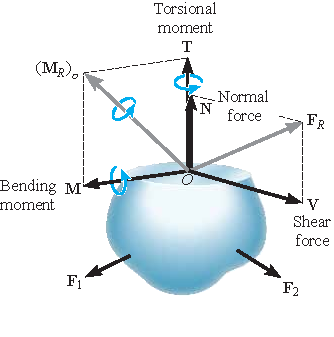
\includegraphics[height = 8cm, keepaspectratio = true]{figures/resultant_loadings.pdf}
    \caption{Resultant loadings acting on a body.}
    % \label{}
\end{figure}
\subsubsection{In 3D}
In 3D, we can represent resultant loadings using four vectors acting over the sectioned area.
\begin{description}
    \item[Normal force] \(\symbf{N}\) force acting perpendicular to the area
    \item[Shear force] \(\symbf{V}\) force acting on an axis tangent to the area
    \item[Torsional moment] \(\symbf{T}\) rotation about the perpendicular axis
    \item[Bending moment] \(\symbf{M}\) rotation about an axis tangent to the area
\end{description}
\subsubsection{In 2D}
In 2D, the body is subjected to a coplanar system of forces, where \(\symbf{T} = \symbf{0}\).
\subsubsection{In 1D}
In 1D, the body is only subjected to axial forces, where \(\symbf{V} = \symbf{T} = \symbf{M} = \symbf{0}\).
\subsection{Stress}
The force and moment acting at a specific point on a sectioned area of a body represent the resultant effects of
the distribution of internal loading that acts over the sectioned area.
\begin{definition}[Stress]
    Consider the quotient of the force \(\Delta \symbf{F}\) over an area \(\Delta A\), then as the \(\Delta A \to 0\),
    so does \(\Delta \symbf{F}\), while the quotient approaches a finite limit. This quotient is called the stress at
    that point.
    \begin{equation*}
        \symbfit{\sigma} = \lim_{\Delta A \to 0} \frac{\Delta \symbf{F}}{\Delta A}
    \end{equation*}
    Here the normal and shear stresses can be expressed using \(\sigma_z\) and \(\tau_{zx}\) and \(\tau_{zy}\).
    \begin{align*}
        \sigma_z  & = \lim_{\Delta A \to 0} \frac{\Delta F_z}{\Delta A} \\
        \tau_{zx} & = \lim_{\Delta A \to 0} \frac{\Delta F_x}{\Delta A} \\
        \tau_{zy} & = \lim_{\Delta A \to 0} \frac{\Delta F_y}{\Delta A}
    \end{align*}

    Stress describes the intensity of the internal force acting on a specific region passing through a point.

    The unit for stress is Pascal where \qty{1}{Pa} or \qty{1}{N.m^{-2}} and \qty{1}{MPa} or \qty{1}{N.mm^{-2}}.
\end{definition}
\subsection{Average Normal Stress}
To determine the average stress distribution acting over a cross-sectional area of an axially loaded bar,
we assume that the material is both \textit{homogeneous} and \textit{isotropic}.
This means the load \(P\) applied through the centroid of the cross-sectional area
will cause the bar to deform uniformly throughout the central region of its length.

By passing a section through a bar, equilibrium requires the resultant normal force \(N\) at the section to be
equal to the external force \(P\). And because the material undergoes a uniform deformation, it is necessary
that the cross section be subjected to a constant normal stress distribution.

As a result, each small area \(\Delta A\) on the cross section is subjected
to a force \(\Delta N = \sigma \Delta A\), where the sum of these forces over the entire cross-sectional area
is \(P\). By letting \(\Delta A \to \odif{A} \) and therefore also \( \Delta N \to \odif{N} \), then as \(\sigma\)
is a constant, we have
\begin{align*}
    \int \odif{N} & = \int_A \sigma \odif{A} \\
    N             & = \sigma A
\end{align*}
Therefore
\begin{equation*}
    \sigma_{\mathrm{avg}} = \frac{N}{A}
\end{equation*}
where in this case \(N = P\).
\begin{theorem}[Equilibrium]
    For an uniaxially loaded body, the equation of force equilibrium gives
    \begin{align*}
        \sigma \left( \Delta A \right) - \sigma' \left( \Delta A \right) & = 0       \\
        \sigma                                                           & = \sigma'
    \end{align*}
    hence the normal stress components must be equal in magnitude but opposite in direction.

    Under this condition, the material is subjected to \textbf{uniaxial stress} and this analysis
    applies to members subjected to tension or compression.
\end{theorem}
\subsection{Strain}
\begin{definition}[Deformation]
    Whenever a force is applied to a body, it will tend to change the body's shape and size.
    These changes are referred to as deformation.
\end{definition}
\begin{definition}[Strain]
    To describe the deformation of a body through changes in lengths of line segments on the surface,
    we will develop the concept of strain.
    If an axial load \(P\) is applied to a bar, it will change the bar's length \(L_0\) to \(L\).
    Then the \textbf{average normal strain} of the bar is defined
    \begin{equation*}
        \epsilon_{\mathrm{avg}} = \frac{L - L_0}{L_0}
    \end{equation*}
    where the numerator is often written as \(\delta = L - L_0\) and is known as elongation or extension.

    The \textbf{normal strain} \(\epsilon\) at a point in a body with an arbitrary shape is defined similarly.
    Consider a small line segment \(\Delta s\) which becomes \(\Delta s'\) after deformation. Then the limit of the normal strain
    is
    \begin{equation*}
        \epsilon = \lim_{\Delta s \to 0} \frac{\Delta s' - \Delta s}{\Delta s}
    \end{equation*}
    In both cases normal strain is positive when the initial length elongates, and negative when the length contracts.

    Strain is a dimensionless quantity sometimes expressed \unit{mm/mm} or \unit{m/m}, or as a percentage.
\end{definition}
\section{Tension and Compression Tests}
To determine the strength of a material, we must perform a tension or commpression test.
This test measures the stress and strain from a load \(P\), and the results can be used to
produce a \textbf{stress-strain diagram}.
There are two ways in which the stress-strain diagram is normally described.
\subsection{Stress-Strain Diagram}
\begin{figure}[H]
    \centering
    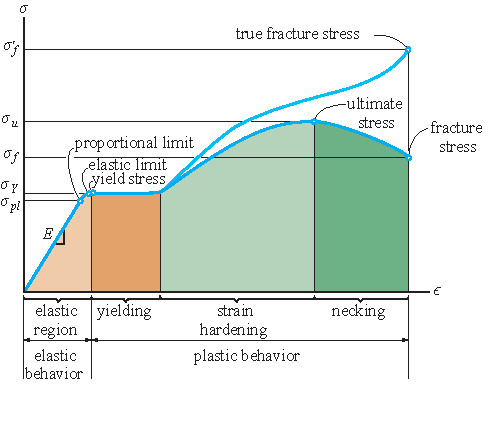
\includegraphics[height = 8cm, keepaspectratio = true]{figures/stress_strain_diagram.pdf}
    \caption{Stress-strain diagram for a typical metal.}
    % \label{}
\end{figure}
\subsubsection{Conventional Stress-Strain Diagram}
The engineering stress assumes that the area \(A\) is constant throughout
the gauge length
\begin{equation*}
    \sigma = \frac{P}{A_0}
\end{equation*}
where \(A_0\) is the \textit{original} cross-sectional area of the specimen.

Likewise, the engineering strain uses the specimen's original length \(L_0\)
\begin{equation*}
    \epsilon = \frac{\delta}{L_0}
\end{equation*}
\subsubsection{True Stress-Strain Diagram}
The true stress and true strain use the instantaneous area \(A\) and length \(L\)
at each measurement.
\subsection{Elastic Behaviour}
The initial region of the curve is referred to as the \textbf{elastic region}
where the deformation is \textit{elastic}, meaning it returns to its original
shape when the load is removed.
\subsubsection{Proportional Limit}
For the majority of the elastic deformation, the curve is \textit{linear}
until the \textbf{proportional limit} \(\sigma_{pl}\).
\subsubsection{Modulus of Elasticity}
As the curve is linear up to \(\sigma_{pl}\), the stress is proportional to the strain.
This is characterised by Hooke's law, and is expressed as
\begin{equation*}
    \sigma = E \epsilon
\end{equation*}
where \(E\) is the constant of proportionality, also called the \textbf{modulus of elasticity}
or \textbf{Young's modulus}.
\subsection{Elastic Limit}
After reaching the proportional limit, the curve bends slightly until it reaches the \textbf{elastic limit}.
\subsection{Plastic Behaviour}
If the stress exceeds the elastic limit, the specimen undergoes \textit{plastic} deformation, meaning
any deformation is permanent.
\subsubsection{Yielding}
The behaviour after elastic deformation is called \textbf{yielding}
and this occurs at the \textbf{yield point} \(\sigma_{Y}\). Any straining
beyond this point will plastically deform the specimen.
\subsubsection{Yield Strength}
Commonly \(\sigma_{pl}\), the elastic limit, and \(\sigma_Y\) occur at the same point,
so a quantity called the \textbf{yield strength} \(\sigma_{YS}\) is defined.

Normally, a 0.2\% strain is chosen, and from this point, a line with gradient \(E\) is drawn.
The point where this line intersects the curve defines \(\sigma_{YS}\).
\subsubsection{Ultimate Tensile Stress}
When yielding has ended, any load causing an increase in stress will be supported by the specimen,
resulting in a curve that rises until it reaches a maximum stress referred to as the \textbf{ultimate stress} \(\sigma_u\).
\subsubsection{Strain Hardening}
This rise in the curve is called \textbf{strain hardening}.
\subsubsection{Necking}
As the specimen elongates up to \(\sigma_u\), its cross-sectional area will decrease in a \textit{uniform} manner over the gauge length.
However after reaching \(\sigma_u\), the cross-sectional area will begin to decrease in a \textit{localised} region where
the stress increases. As a result, a ``neck'' forms at this region, and the specimen experiences \textbf{necking}.
\subsubsection{Fracture Stress}
Finally, the specimen breaks at the \textbf{fracture stress} \(\sigma_f\) at the end of the downward curve.
\subsection{Ductility}
\begin{definition}[Ductility]
    Ductility is a measure of the amount of plastic deformation a material can sustain under tensile stress before failure.

    Ductility can be measured using its \textbf{percent elongation} (in length) or \textbf{percent reduction} (in area).

\end{definition}
\subsection{Brittleness}
\begin{definition}[Brittleness]
    Brittleness describes the
\end{definition}
\subsection{Poisson's Ratio}
When a deformable body is subjected to a force, it can elongate longitudinally and also contract laterally.
The strain in the longitudinal (or axial) direction is given by
\begin{equation*}
    \epsilon_{\mathrm{long}} = \frac{\delta}{L}
\end{equation*}
and the strain in the lateral (or radial) direction is given by
\begin{equation*}
    \epsilon_{\mathrm{lat}} = \frac{\delta'}{r}
\end{equation*}
where \(\delta'\) is the change in the radius \(r\).

Consider the ratio of these two quantities \(\nu\)
\begin{equation*}
    \nu = -\frac{\epsilon_{\mathrm{lat}}}{\epsilon_{\mathrm{long}}}.
\end{equation*}
Within the elastic region, this quantity will be constant, and it is referred
to as \textbf{Poisson's ratio}.

Note the negative value is introduced as the lateral axis contracts.
\end{document}
